Растровый рисунок использует сеточное заполнение цветом. Из-за этого при изменение разрешения изображения картинка приобретает
резкий вид, связанный с наблюдением резкой сетки заместо плавного изображения.

Тем не менее такой вид искусства популярен в силу простоты освоения и восприятия. Интерактивная игра предлагает 

Для отображения используется открытая диффузионная модель \ref{diffusion} для составления рисунка по текстовому запросу. 



Для выполнения рисунка она получает запрос на английском языке, лаконично описывающий стиль рисования и объекты на изображении.
В силу случайности генерации пользователь может подобрать для себя наиболее интересный вариант изображения.

Модель дополнительно снабжена фильтром цензуры, позволяющей избегать неэтичного рисунка \cite{radford2021learning}.

\begin{figure}[h]
    \centering
    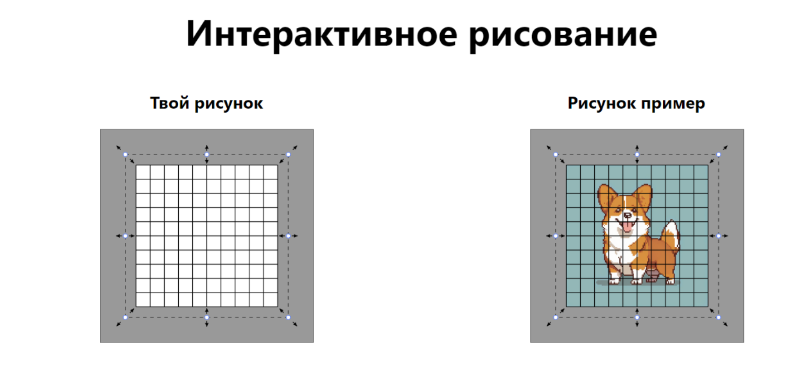
\includegraphics[width=0.5\textwidth]{assets/work/games/draw.excalidraw.png}
    \caption{Сложность задания задается организацией рисунка}
    \label{draw}
\end{figure}


Ассистент выполняет задачи \begin{itemize}
    \item транслирует запрос пользователя на русском языке на английский для генерации
\end{itemize}



Уровень сложности регулируется путем изменения композиции и наличия фона.


